\documentclass[a4paper]{article}

%use the english line for english reports
%usepackage[english]{babel}
\usepackage[portuguese]{babel}
\usepackage[utf8]{inputenc}
\usepackage{indentfirst}
\usepackage{graphicx}
\usepackage{verbatim}
\usepackage[margin=1.0in]{geometry}
\usepackage{listings}

\begin{document}
\renewcommand{\figurename}{Fig.}

\setlength{\textwidth}{16cm}
\setlength{\textheight}{22cm}

\title{\Huge\textbf{Nodes}\linebreak\linebreak\linebreak
\Large\textbf{Relatório Intercalar}\linebreak\linebreak
\linebreak\linebreak

\includegraphics[scale=0.1]{feup-logo.png}\linebreak\linebreak
\linebreak\linebreak
\Large{Mestrado Integrado em Engenharia Informática e Computação} \linebreak\linebreak
\Large{Programação em Lógica}\linebreak
}

\author{\textbf{Grupo Nodes\_3:}\\
Carolina Centeio Jorge - up201403090 \\
Tiago Almeida - up201305665 \\
\linebreak\linebreak \\
 \\ Faculdade de Engenharia da Universidade do Porto \\ Rua Roberto Frias, s\/n, 4200-465 Porto, Portugal \linebreak\linebreak\linebreak
\linebreak\linebreak\vspace{1cm}}

\maketitle
\thispagestyle{empty}

%************************************************************************************************
%************************************************************************************************

\newpage

%Todas as figuras devem ser referidas no texto. %\ref{fig:codigoFigura}
%
%%Exemplo de código para inserção de figuras
%%\begin{figure}[h!]
%%\begin{center}
%%escolher entre uma das seguintes três linhas:
%%\includegraphics[height=20cm,width=15cm]{path relativo da imagem}
%%\includegraphics[scale=0.5]{path relativo da imagem}
%%\includegraphics{path relativo da imagem}
%%\caption{legenda da figura}
%%\label{fig:codigoFigura}
%%\end{center}
%%\end{figure}
%
%
%\textit{Para escrever em itálico}
%\textbf{Para escrever em negrito}
%Para escrever em letra normal
%``Para escrever texto entre aspas''
%
%Para fazer parágrafo, deixar uma linha em branco.
%
%Como fazer bullet points:
%\begin{itemize}
	%\item Item1
	%\item Item2
%\end{itemize}
%
%Como enumerar itens:
%\begin{enumerate}
	%\item Item 1
	%\item Item 2
%\end{enumerate}
%
%\begin{quote}``Isto é uma citação''\end{quote}


%%%%%%%%%%%%%%%%%%%%%%%%%%
\section{Nodes: The Game}

\subsection{History}

Nodes is a board game of abstract strategy, created by The Game Crafter and designed by RGBY Games. It was released on September 10, 2016 and it is still on its 1st edition. This game was made for casual gamers, in particular, for people who like chess due to their similarity. Nodes require 2 to 4 players over the age of 12.


\subsection{Brief Description}

\subsubsection{Pieces}

\textbf{Nodes:} Each player starts with \textbf{1} node. Nodes are like kings in chess: they can only move \textbf{one space in each turn}. In this game, they are also communication hubs. They emit signals in all eight directions (front, back, sides and diagonals), called \textbf{lines of communication}.
\newline

\textbf{Units:} Each player starts with \textbf{8} units. Unlike pawns in chess, units can move as many spaces as they want in each turn, \textbf{as long as they are along} a line of communication.

\begin{figure}[h!]
	\centering
	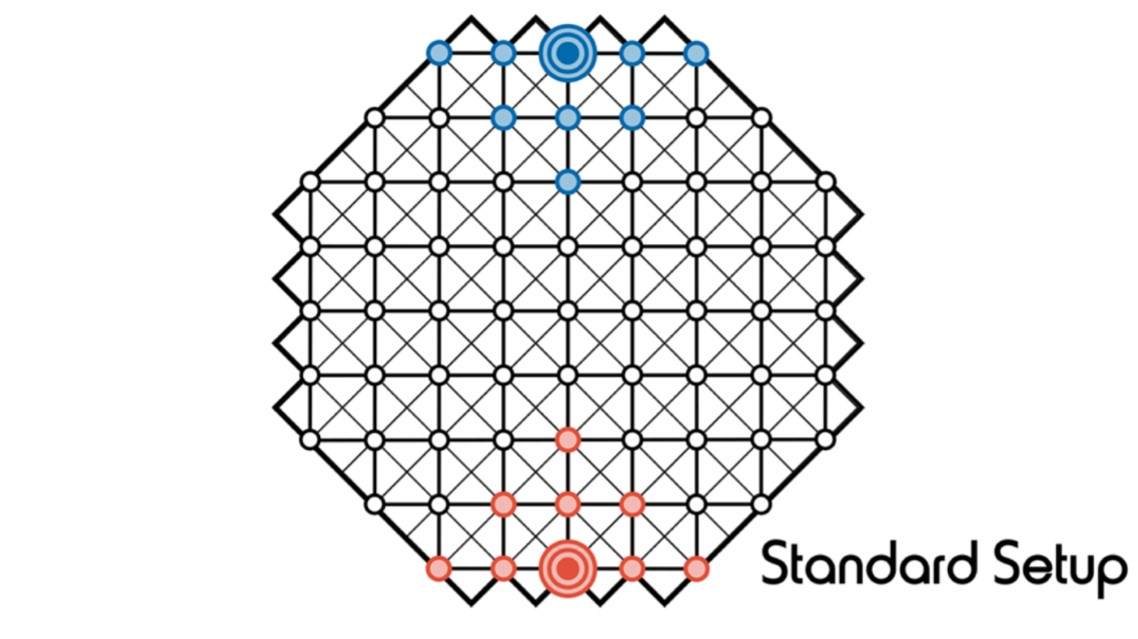
\includegraphics[width=0.5\textwidth]{boardinit.jpg}
	\caption{Initial board set up}
	\label{Image: Initial board set up}
\end{figure}

\subsubsection{Board}
\begin{figure}[!h]

\centering
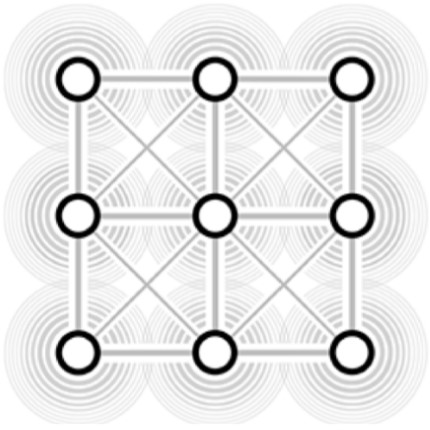
\includegraphics[width=.2\textwidth]{spaces.jpg}
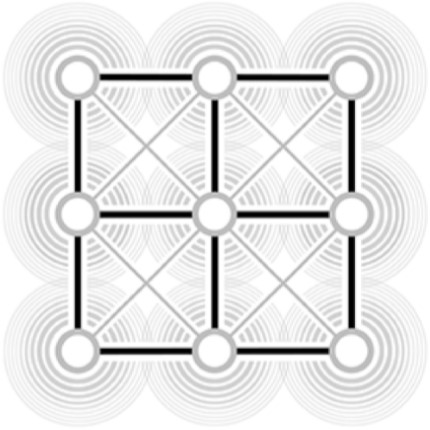
\includegraphics[width=.2\textwidth]{roads.jpg}
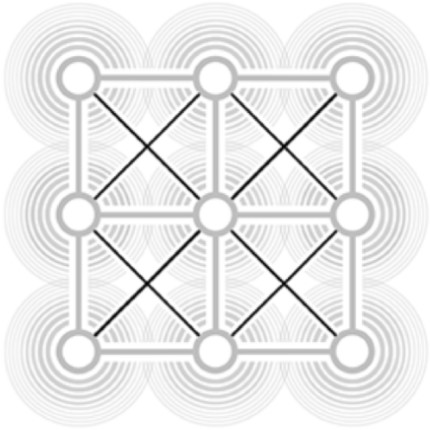
\includegraphics[width=.2\textwidth]{conduits.jpg}

\caption{Spaces, Roads and Conduits}
\label{fig:figure3}

\end{figure}

\textbf{Spaces: }White circles where both units and nodes can finish their turn.

\textbf{Roads: }Boldest lines connecting spaces along which both pieces can draw their paths.

\textbf{Conduits: }Thin crossing lines that cannot be part of a piece's path.


\subsection{Rules}

\subsubsection{Lines of Communication}

Lines of communication are the basis of the movement. Each node emits a line of communication along each road and conduit that surrounds it. All lines of communication are available in every player's turn, even if they are being emitted by another player's node. 
Relay and Interception?


\subsubsection{Unit Movements}

Units can move through communication lines until the player decides to finish its turn. They cannot move through conduits. There is no limit on how many spaces a unit can move.
Under some circumstances, it is possible for a unit to jump over another one. This can happen when when the spaces before and after the unit in the way are in the same line of communication: units cannot jump over nodes and can only jump one enemy unit at a time.



\subsubsection{How to play}
Each turn has three stages. The first one consists in visualizing the line of communication and determine which units can move. Then, the player moves each unit to the desired position (if possible).
\begin{figure}[h!]
	\centering
	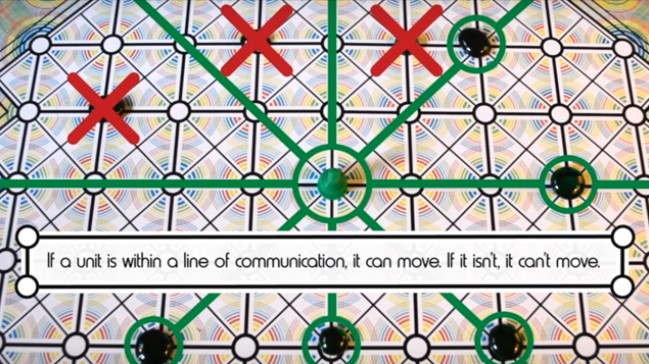
\includegraphics[width=0.5\textwidth]{signallines.jpg}
	\caption{In green, the communication Lines. Units with a circle can move. Units with a cross cannot.}
	\label{Image: signallines}
\end{figure}


%Descrever detalhadamente o jogo, a sua história e, principalmente, as suas regras.
%Devem ser incluidas imagens apropriadas para explicar o funcionamento do jogo.
%Devem ser incluidas as fontes de informação (e.g. URLs em rodapé).


%%%%%%%%%%%%%%%%%%%%%%%%%%
\section{Representation of the Game State}

The board is composed of a list of lists (representing each line) of lists (margin and content). This is a two player game representation.

It is an octagonal board and it uses units and nodes with the number of the player (ex: unit1 and node1 are an unit and a node of the player one. They are represented as 'x' and '1', respectively. For player 2, there are 'o' for units and '2' for the node). 

This is the code that describes the different stages of the game (images follow):

\textbf{Initial Formation:}

\begin{lstlisting}

board( [[[null,roof], [unit1,unit1,node1,unit1,unit1]],
       [[roof], [empty,empty,unit1,unit1,unit1,empty,empty]],
       [[], [empty,empty,empty,empty,unit1,empty,empty,empty,empty]],
       [[], [empty,empty,empty,empty,empty,empty,empty,empty,empty]],
       [[], [empty,empty,empty,empty,empty,empty,empty,empty,empty]],
       [[], [empty,empty,empty,empty,empty,empty,empty,empty,empty]],
       [[], [empty,empty,empty,empty,unit2,empty,empty,empty,empty]],
       [[null], [empty,empty,unit2,unit2,unit2,empty,empty]],
       [[null,null], [unit2,unit2,node2,unit2,unit2]]]).
\end{lstlisting}

\begin{figure}[h!]
	\centering
	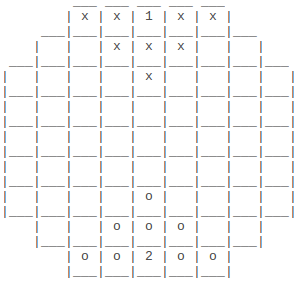
\includegraphics[width=0.3\textwidth]{InitialFormation.png}
	\caption{Initial formation for 2 players.}
	\label{Image: initformation}
\end{figure}

\textbf{Middle Stage:}

\begin{lstlisting}

board( [[[null,roof], [empty,empty,empty,empty,empty]],
       [[roof], [empty,empty,empty,empty,empty,empty,empty]],
       [[], [empty,empty,empty,empty,unit1,empty,empty,empty,empty]],
       [[], [empty,empty,empty,unit2,unit2,empty,empty,empty,empty]],
       [[], [empty,node2,unit2,unit2,unit1,unit2,unit2,empty,empty]],
       [[], [empty,unit2,unit1,unit1,empty,empty,empty,unit2,empty]],
       [[], [unit1,unit1,unit1,empty,node1,empty,empty,empty,empty]],
       [[null], [empty,unit1,empty,empty,empty,empty,empty]],
       [[null,null], [empty,empty,empty,empty,empty]]]).
\end{lstlisting}

\begin{figure}[h!]
	\centering
	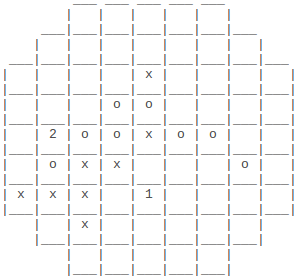
\includegraphics[width=0.3\textwidth]{MidGame.png}
	\caption{An example of a middle game stage.}
	\label{Image: midgame}
\end{figure}

\textbf{Final Stage:}

\begin{lstlisting}

board( [[[null,roof], [empty,empty,empty,empty,empty]],
       [[roof], [empty,empty,empty,empty,empty,empty,empty]],
       [[], [empty,empty,empty,empty,unit1,empty,empty,empty,empty]],
       [[], [empty,unit1,unit1,unit2,empty,empty,empty,empty,empty]],
       [[], [unit1,empty,node2,empty,empty,empty,empty,empty,empty]],
       [[], [unit1,unit2,unit1,empty,empty,empty,unit2,unit2,empty]],
       [[], [empty,unit1,empty,empty,unit2,empty,empty,empty,empty]],
       [[null], [empty,unit1,unit2,node1,unit2,empty,empty]],
       [[null,null], [empty,empty,unit2,empty,empty]]]).
\end{lstlisting}


\begin{figure}[h!]
	\centering
	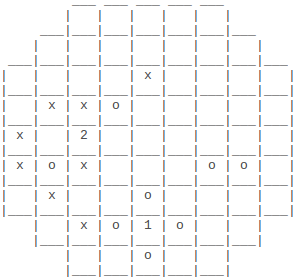
\includegraphics[width=0.3\textwidth]{FinalGame.png}
	\caption{Final stage: Node 1 surrounded.}
	\label{Image: finalgame}
\end{figure}

%Descrever a forma de representação do estado do tabuleiro (tipicamente uma lista de listas), com exemplificação em Prolog de posições iniciais do jogo, posições intermédias e finais, acompanhadas de imagens ilustrativas.


%%%%%%%%%%%%%%%%%%%%%%%%%%
\section{Board Preview}

In this octagonal board, each square represents a \textbf{space}. In the original game, spaces are vertexes. For this reason, roads and conduits are not represented.

The board will be displayed with the \textbf{displayBoard(X)} predicate. This predicate draws the top of the board and calls the \textbf{displayBoardAux(X)} predicate which will display the lines. The \textbf{displayLine(X)} predicate draws the margins (\textbf{displayLineMargin(X)}), the content of the line (positions and its content: \textbf{displayLineContent(X)}) and the borders of the lines and board (\textbf{displayLineBottom(X)}, \textbf{displayLineMarginBottomLeft(X)} and \textbf{displayLineMarginBottomLeft(X)}).

\begin{lstlisting}
translateContent(empty, '   ').
translateContent(unit1, ' x ').
translateContent(unit2, ' o ').
translateContent(node1, ' 1 ').
translateContent(node2, ' 2 ').
translateContent(roof, '    ').
translateContent(null, '    ').
translateBottom(X, '') :-
       member(X, [empty, unit1, unit2, node1, node2]).
translateBottomLeft(roof, ' ___').
translateBottomLeft(null, '    ').
translateBottomRight(roof, '___').
translateBottomRight(null, '    ').

displayLineMargin([]) :-
       write('').

displayLineMargin([LF1|LFs]) :-
       translateContent(LF1, V),
       write(V),
       displayLineMargin(LFs).

displayLineMarginBottomLeft([]):-
       write('').

displayLineMarginBottomLeft([LF1|LFs]) :-
       translateBottomLeft(LF1, V),
       write(V), 
       displayLineMarginBottomLeft(LFs).

displayLineMarginBottomRight([]):-
       write('').

displayLineMarginBottomRight([LF1|LFs]) :-
       translateBottomRight(LF1, V),
       write(V), 
       displayLineMarginBottomRight(LFs).

displayLineContent([]) :-
       write('|'),
       nl.

displayLineContent([LF1|LFs]) :-
       translateContent(LF1, V),
       write('|'),
       write(V),
       displayLineContent(LFs).

displayLineBottom([]) :-
       write('|').

displayLineBottom([LF1|LFs]) :-
       translateBottom(LF1, V),
       write(V), 
       write('|___'),
       displayLineBottom(LFs).

displayLine([]) :-
       write('').

displayLine([E1|Es]):-
       displayLineMargin(E1),
       member(X, Es),
       displayLineContent(X),
       displayLineMarginBottomLeft(E1),
       member(X, Es),
       displayLineBottom(X),
       reverse(E1, Y),
       displayLineMarginBottomRight(Y),
       nl.      

displayBoardAux([]) :-
       displayLine([]).

displayBoardAux([L1|Ls]):-
       displayLine(L1),
       displayBoardAux(Ls).

displayBoard(X) :-
       write('         ___ ___ ___ ___ ___'),
       nl,
       displayBoardAux(X).
\end{lstlisting}

\begin{figure}[h!]
	\centering
	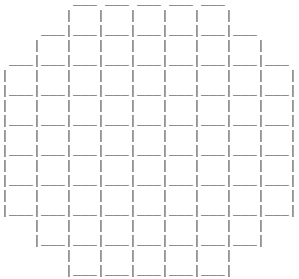
\includegraphics[width=0.3\textwidth]{Board.png}
	\caption{Empty Board.}
	\label{Image: board}
\end{figure}
%Descrever a forma de visualização do tabuleiro em modo de texto e o(s) predicado(s) Prolog construídos para o efeito.
%Deve ser incluída pelo menos uma imagem correspondente ao output produzido pelo predicado de visualização.


%%%%%%%%%%%%%%%%%%%%%%%%%%
\section{Moves}

In each turn, players can move as many pieces as they want. For this to happen, there will be the following predicates:

\begin{lstlisting}
up(+Board, +Player, -NewBoard).
down(+Board, +Player, -NewBoard).
right(+Board, +Player, -NewBoard).
left(+Board, +Player, -NewBoard).
\end{lstlisting}

%Elencar os movimentos (tipos de jogadas) possíveis e definir os cabeçalhos dos predicados que serão utilizados (ainda não precisam de estar implementados).

\end{document}
